\documentclass[12pt, a4paper, twoside, openright]{book}

\usepackage[french]{babel}
\usepackage[T1]{fontenc}
\usepackage[utf8]{inputenc}
\usepackage{lmodern}
\usepackage{graphicx}
\usepackage{hyperref}
\usepackage{listings}
\usepackage{graphicx}
\usepackage{microtype}
\usepackage{glossaries}
\usepackage{color}
\usepackage{here}
\usepackage{float}

\makeglossaries %à la suite de la déclaration de package
\newacronym{sgbd}{Système de gestion de base de données}{Logiciel permettant...}



%define
\newcommand{\fontconsolas}[1]{\fontfamily{pag}\selectfont 
#1
}

\newcommand{\exemple}[1]{\newline\newline
\begin{center}
\parbox{10cm}{\textcolor[rgb]{0.5,0.5,0.5}{\fontconsolas{#1}}}
\end{center}
}

\newcommand{\sgbd}{\textbf{Système de Gestion de Base de Données}}
%end define


\title{Interface homme-machine pour gestion de bases de données.}
\author{ALCANTUD Gaël \\ BULATOVIC Alexandre \\ MAURY Adrian \\ UGOLINI Romain \\ \\tuteur : PALLEJA Xavier}
\date{20/02/2017}


\begin{document}
\frontmatter
\maketitle

%\thispagestyle{empty}
%\chapter*{Résumé}
%\textbf{IDB} est un logiciel gratuit permettant d'utiliser un SGBD* au moyen d'une interface graphique. Son interface est intuitive et permet à un utilisateur, même non informaticien, de manipuler très facilement des tables et les données qu'elles contiennent, mais aussi d'effectuer des requêtes simples (en allant jusqu'aux jointures) sans se soucier du langage SQL*.
\\
Le logiciel est entièrement codé en langage Java (nécessite au minimum JRE* 1.7) et se base sur la bibliothèque JDBC* pour réaliser la communication avec la base de données. Il est entièrement compatible avec les système de gestion de base de données Oracle Database et MySQL.
\bigbreak
Mots clés : base de données, JAVA, JDBC, SQL, interface graphique, Oracle, MySQL, QBE

\bigbreak
\rule{\linewidth}{0.4pt}
\bigbreak

\textbf{IDB} is a free software intended to handle the administration of a database management system with the use of a GUI*. Its use is intuitive and allow non-IT people to manage tables and their data, but also to perform simple queries (even join clause) without having to know SQL*.
\\
This software is written in Java language (requires JRE* 1.7+) and uses the JDBC* tool from Java language to achieve communication with the database management system. It's fully compatible with Oracle Database and MySQL.
\bigbreak
Keywords : database, JAVA, JDBC, SQL, graphical user interface, Oracle, MySQL, QBE


\thispagestyle{empty}
\chapter*{Remerciements}



Premièrement nous tenons à remercier notre tuteur de projet, \textbf{M. Xavier PALLEJA}, pour avoir encadré ce projet et nous avoir guidé dans la réalisation de l'application à l'aide d'un cycle de développement itératif.

Nous apprécions grandement sa forte implication dans le projet et nous tenons à lui en faire part.

\bigbreak

Nous remercions également les différentes personnes travaillant à l'IUT nous ayant permis d'avancer le projet en mettant à disposition des salles informatiques, notamment les techniciens réseau.

\bigbreak
Enfin, nous remercions \textbf{M. Francis GARCIA} pour son rôle de chef de département informatique et d'avoir fait en sorte que tout se passe au mieux.

De même nous remercions notre professeur de communication \textbf{M. Alain RAIBAUT} pour ses cours qui nous ont été utile à la rédaction de ce rapport ainsi que les précieux conseils donnés sur la façon de gérer une présentation orale.


\tableofcontents
\listoffigures
\printglossaries

\mainmatter
\chapter{Introduction}
Les \glspl{bdd} sont des outils permettant de stocker et retrouver des \glspl{data}, c'est à dire des valeurs brutes. 
Ces outils se trouvent au coeur des \glspl{si}, et sont indispensables aux entreprises.

En informatique, les bases de données sont numérisées, définies et manipulées grâce à des logiciels nommés \glspl{sgbd}.

Il existe différents types de bases de données, mais le marché reste dominé par les \glspl{bddr}\footnote{\label{part_de_marché_relationnel}
Classement des \glspl{sgbd} les plus populaires : \url{http://db-engines.com/en/ranking}}. Ces dernières sont gérées par des SGBD relationnels (dit SGBDR) 
dont les plus connus sont Oracle, MySQL et PostgreSQL.

Ces logiciels permettent de définir et de manipuler des bases de données par le biais du \gls{sql}, 
langage déclaratif et normé qui reste le premier et le plus exhaustif des moyens de gérer une base de données relationnelle .

Mais le SQL est un langage informatique, ce qui constitue un frein pour les utilisateurs : s'ils ne connaissent pas
le langage, ils ne peuvent pas utiliser de base de données.

Certaines applications, comme \textit{Access}, \textit{LOBase} ou encore \textit{phpMyAdmin} proposent une alternative au SQL grâce à des 
\glspl{ihm}: il est possible de définir les données ou de les manipuler par des clics de boutons, des glisser-déplacer, des cases à cocher ou encore de la saisie
de texte non codé. 

En suivant cette optique, le but de ce projet tuteuré est de réaliser une application permettant d'utiliser certaines fonctionnalités 
des bases de données \underline{sans} 
avoir recours au SQL, et ce sur n'importe quel SGBDR. Pour cela, elle propose une série d'IHM qui en reprennent certaines fonctionnalités,
à savoir le \gls{ldd} et le \gls{lmd}.

Les utilisateurs finaux de l'application sont les élèves de première année du DUT Informatique, pour
les aider à découvrir les bases de données.

Ce document présente les différentes phases de création de cette application : l'analyse, la conception, le développement et les tests.
Un manuel d'utilisation est disponible dans les dernières pages.

Afin de mieux situer l'application, la figure \ref{sans_idb_schema} montre l'utilisation classique d'un SGBD et 
la figure \ref{avec_idb_schema} l'utilisation de l'application développée.

\begin{figure}[!h]
  \centering
  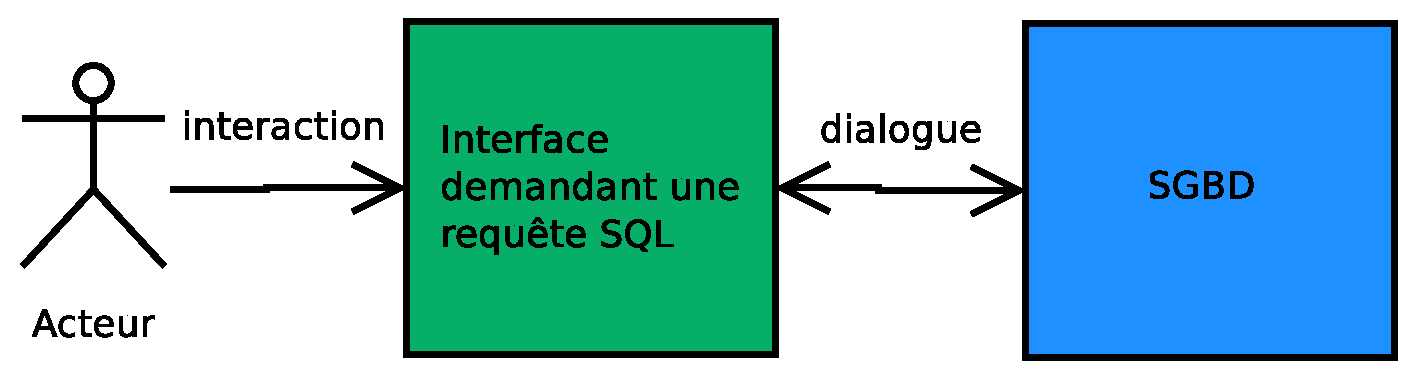
\includegraphics[width=14cm]{images/sans_idb.eps}
  \caption{Utilisation classique d'un SGBD.}
  \label{sans_idb_schema}
\end{figure}

\begin{figure}[!h]
  \centering
  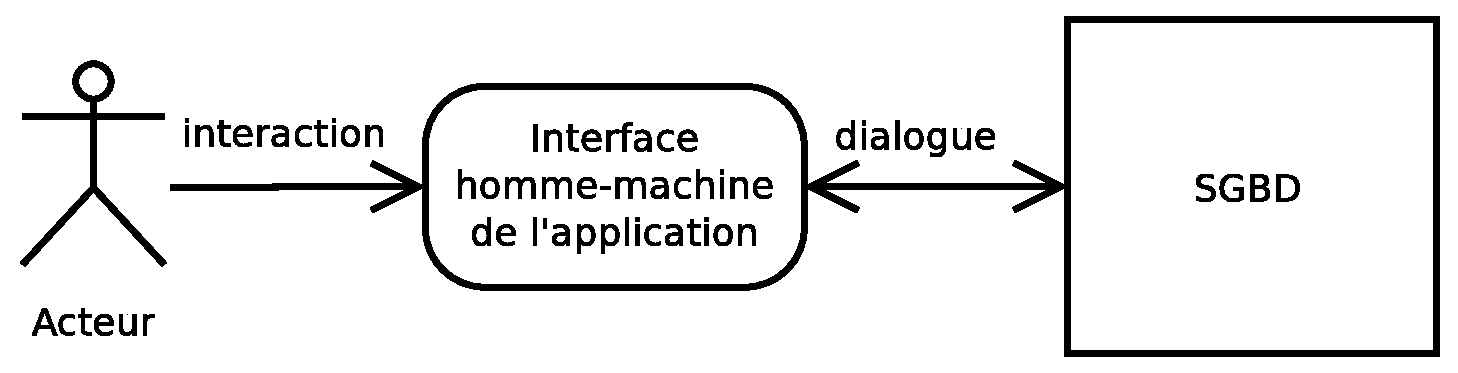
\includegraphics[width=14cm]{images/avec_idb.eps}
  \caption{Utilisation d'un SGBD avec l'application du projet.}
  \label{avec_idb_schema}
\end{figure}
%TODO : donner un nom à l'application


\chapter{Analyse}
\section{Contexte}
Comme mentionné précédemment, les SGBDR sont les plus utilisés des \glspl{sgbd}. Ils permettent de manipuler des bases de données relationnelles
par le biais du langage \gls{sql}. Puisque ce langage nécessite un certain apprentissage, un utilisateur ne le connaissant pas ne peut pas se servir
d'une base de données.

Ce projet tuteuré demande le développement d'une application permettant d'utiliser une base de données :
\begin{itemize}
\item sans utiliser le SQL,
\item compatible avec n'importe quel SGBD.
\end{itemize}


\section{Fonctionnalités}
L'application propose des fonctionnalités des SGBD vues durant le cursus à l'IUT.
Un exemple de requête SQL est indiqué pour chaque fonctionnalité.
L'utilisateur n'a pas à écrire ces codes pour gérer sa base de données.

\subsection{Le Langage de Définition des Données (LDD)}
Le langage de définition des données permet de structurer une base de données.
Il ne s'intêresse pas aux données contenues dans les tables
\footnote{\label{interet_ldd}Le LDD prend en compte les données contenues dans les tables et peut agir dessus, mais c'est une conséquence, pas son rôle.}, mais aux tables elles même. Le LDD est séparé en trois instructions:

\subsubsection{Create table}
Permet de créer une \gls{table}. Dans un SGBD, les tables sont nommées, chaque nom est unique.
Une table est créée avec au moins un attribut dont il faut préciser le type de données (texte, nombre, date etc.) et la taille.
Des \glspl{constraint} supplémentaires peuvent être ajoutées : les \textit{\glspl{primarykey}} \footnote{\label{contrainte_clée_primaire}Voir glossaire.}, les attributs \textit{not null} et groupes d'attributs \textit{uniques}.

La \gls{query} suivante montre la création d'une table nommée PERSONNES, qui contient les attributs \textit{idpersonne}, \textit{nompersonne}, \textit{taillepersonne} et \textit{datenaissancepersonne}.

  \begin{lstlisting}
    CREATE TABLE PERSONNES
    (
    idpersonne CHAR(5),
    nompersonne VARCHAR(30),
    taillepersonne NUMBER,
    datenaissancepersonne DATE
    );
  \end{lstlisting}

\subsubsection{Alter table}
Permet de revenir sur ce qui a été fait avec CREATE TABLE.
L'instruction permet d'ajouter, supprimer ou modifier des \glspl{attribut}, des contraintes, des index...

Cette instruction se comporte différemment selon qu'une table soit vide ou remplie de lignes de données (\glspl{tuple}).
Par exemple, ajouter une contrainte NOT NULL sur une colonne possédant déjà des tuples nuls n'est pas possible. Ce problème n'existe pas sur une table vide.

La requête SQL suivante modifie la table \textit{PERSONNES} pour y ajouter une contrainte de clée primaire nommée \textit{pk\_personnes} sur l'attribut \textit{idpersonne}.

\begin{lstlisting}
  ALTER TABLE PERSONNES
  (
  ADD CONSTRAINT pk_personnes PRIMARY KEY (idpersonne)
  );
\end{lstlisting}

\subsubsection{Drop table}
Permet de supprimer une table et les données qu'elle contient.
Dans une base de données relationnelles, les tables sont liées entre elles par des attributs.
La supression d'une table peut entraîner la supression de données dans d'autres tables, en fonction du schéma relationnel de la base.

La requête SQL suivante supprime la table \textit{PERSONNES} de la base de données.
\begin{lstlisting}
  DROP TABLE PERSONNES;
\end{lstlisting}

\subsection{Le Langage de Manipulation des Données (LMD)}
Le langage de manipulation des données permet d'affectuer des actions de \gls{crud} sur ce que contiennent les tables.
En d'autres termes, il agit sur les tuples.

\subsubsection{Create}
Il d'agit de créer un nouveau tuple dans une table.
La requête SQL suivante permet d'ajouter un tuple de clée primaire \textit{00001} dans la table \textit{PERSONNES}.
\begin{lstlisting}
  INSERT INTO PERSONNES
  (idpersonne, nompersonne, taillepersonne,
  datenaissancepersonne)
  VALUES
  ('00001', 'DUPONT', 'Jean', '06/08/1985');
\end{lstlisting}

\subsubsection{Read}
Il s'agit de récupérer, lire, croiser des données que contiennent les tables.
Les requêtes SQL  "read" peuvent être très complexes.
Certains SGBD proposent des \glspl{qbe}
\footnote{Access, LOBase, phpMyAdmin...}pour créer ces requêtes sans manipuler de SQL.
Celle qui est écrite juste après est simple et permet de retrouver le nom de la \textit{PERSONNES} numéro "00001".
\begin{lstlisting}
  SELECT PERSONNES.nompersonne
  FROM PERSONNES
  WHERE PERSONNES.idpersonne = '00001';
\end{lstlisting}

\subsubsection{Update}
Il s'agit de modifier un ou plusieurs tuples qui existent déjà dans la table.
La requête SQL suivante remplace le nom de famille de la \textit{PERSONNES} "00001" par "Robert".
\begin{lstlisting}
  UPDATE PERSONNES
  SET nompersonne = 'Robert'
  WHERE idpersonne = '00001';
\end{lstlisting}

\subsubsection{Delete}
Il s'agit de supprimer un ou plusieurs tuples.
La requête SQL suivante supprime les tuples des \textit{PERSONNES} qui s'appellent "Jean".
\begin{lstlisting}
  DELETE FROM PERSONNES
  WHERE prenompersonne = "Jean";
\end{lstlisting}

\subsection{Le Langage de Controle des Données (LCD)}
Cet aspect du SQL n'est pas demandé pour l'application et n'est pas traité.

\subsection{Transaction ACID}
Cet aspect des bases de données n'est pas demandé pour l'application et n'est pas traité.
En d'autres termes, une base de données géré par l'application ne peut être utilisée que par une seule personne à fois, sinon elle perd sa cohérence.

\subsection{Résumé des fonctionnalités}
L'application permet de :
\begin{itemize}
\item créer une table,
\item modifier une table,
\item supprimer une table,
\item ajouter des tuples,
\item croiser des données,
\item modifier des tuples,
\item supprimer des tuples.
\end{itemize}

Les fonctionalités précédentes sont utilisables sans connaissance du SQL.


\section{Besoins non-fonctionnels}

\subsection{Systèmes d'exploitation}
L'application fonctionne sur les systèmes d'exploitation Windows XP, Windows 7 et Ubuntu.

\subsection{Version du Java Runtime Environment}
L'application fonctionne avec une version de JRE supérieur ou égale à la version 1.7 (la version présente à l'IUT).

\subsection{Interfaces Homme-Machine (IHM)}
L'application fournit des IHM pour manipuler les bases de données sans utiliser le langage SQL.
Elles sont ergonomiques, non boguées et limitent les actions, empêchant l'utilisateur de faire des erreurs.

L'application suit les patterns habituels des applications possédant des vues :
application en couche ou \gls{MVC}*.

\subsection{Performances}
L'application ne doit pas être lente, malgré sa connexion à distance avec le SGBD.

\subsection{Compatibilité avec les SGBD}
Il existe plusieurs SGBD sur le marché.
L'application peut être utilisée sur plusieurs SGBD distincts.
Elle doit se comporter de la même façon quelque soit le SGBD utilisé.

Il n'est pas demandé que l'application soit connectée à plusieurs SGBD en \textit{même temps}.



\chapter{Conception}\label{chapitre_conception}
\section{Réponse aux besoins non-fonctionnels}
Choix effectués pour répondre aux besoins non-fonctionnels.

\subsection{Systèmes d'exploitation}
L'application est développée avec le langage Java, pour profiter des \textit{machines virtuelles} qui permettent d'utiliser l'application sur n'importe quel système d'exploitation ayant une version du \gls{JRE}* installée
\footnote{\label{les_machines_virtuelles}Machines virtuelles Java : \url{https://docs.oracle.com/javase/8/docs/technotes/guides/vm/}}.

\subsection{Version du Java Runtime Environment}
L'\gls{IDE}* est configuré de façon à utiliser la version 1.7 de \gls{JRE}*.

\subsection{Interfaces Homme-Machine (IHM)}
Les IHM sont développées en Java, en utilisant les classes des packages \textit{java.swing} et \textit{javax.swing}. Ces packages disposent des listes déroulantes, cases à cocher, boutons, barre de défilements, etc.
\footnote{\label{element_de_formulaire}Package \textit{javax.swing} : \url{https://docs.oracle.com/javase/7/docs/api/javax/swing/package-summary.html}}.

\subsection{Performances}
Pour éviter les lenteurs dues aux accès vers le SGBD, l'application possède une couche \gls{orm} sur les tables.

\subsection{Compatibilité avec les SGBD}
L'application est conçue sur le principe \underline{ouvert-fermé} : pour la rendre compatible avec un nouveau SGBD, il n'y a que du code à \textit{ajouter}, aucun (ou presque) à \textit{modifier}.


\section{Les classes métiers}
\subtitle{Les classes métiers}
Il nous a été nécessaire de créer des classes métiers représentant fidèlement le comportement 

\begin{figure}[!h]
\centering
\includegraphics[width=14cm]{./images/metiers.eps}
\caption{Diagramme de classes métiers}
\label{classes_metiers}
\end{figure}


Ces classes ont une particularité, c'est de pouvoir générer du SQL à partir de leurs attributs ou de différents arguments.
Lorsqu'une table est supprimé, tous les attributs de la table sont détruits et toutes les contraintes composant les attributs et la table sont détruit également.
Si un seul attribut est détruit, toutes les contraintes qui le compose sont détruites, ainsi, une contrainte \textbf{ForeignKeyConstraint} sera détruit même si elle concerne un second attribut
\exemple{une fk1 composé de att1 et att2 pointant sur pk1 et pk2 respectivement. L'on supprime att1, alors la clé étrangère ne peut pas respecter la norme et la constrainte fk1 est supprimé}\label{section_metiers}


\chapter{Les Tests}
Les tests constituent des éléments indispensables, ils permettent d'avancer sur un projet sans que les nouvelles implémentations ne viennent modifier le comportement existant.
\section{Pourquoi tester}


Idéalement, chaque classe devrait être testé \textbf{unitairement}.
Malheureusement, certains comportement ne peuvent pas être testé de manière efficiente (= de façon automatique) car par exemple pour tester les fonctionnalités d'un logiciel ayant des interactions avec \gls{sgbd}, il faudrait que l'utilisateur stocke ses identifiants de connexion en dur dans une classe accessible par sa classe de test, et il faudrait également qu'il ait préalablement créé la liste de toutes les tables nécessaires au fonctionnement de son programme.
\bigbreak

Pour pallier à ce problème, il est possible de créer une deuxième classe avec les comportements attendus directement introduits par le développeur (c'est-à-dire que si la classe normale doit effectuer une vérification sur un système externe et retourner \textit{true} ou \textit{false} selon le résultat de cette vérification, la classe mock, elle, retournera directement \textit{true} ou \textit{false} sans faire de vérifications, c'est ce que l'on appelle "\underline{mocker la classe}"). L'inconvénient de cette façon de faire est que cela agrandit considérablement le nombre de classes Java du projet.


\bigbreak
  Heureusement, il existe des bibliothèques externes qui permettent de créer des objets \gls{mock}* sans avoir à créer une nouvelle classe.
Les classes natives de Java ne seront pas "mocké" car celles-ci ont déjà été testées avant d'être intégrées à Java et sont donc considérées "parfaites" (sans bugs).
\bigbreak
Exemple d'utilisation de la bibliothèque externe \textit{Mockito} :

\lstset{
language=Java,
basicstyle=\normalsize, % ou ça==> basicstyle=\scriptsize,
upquote=true,
aboveskip={1.5\baselineskip},
columns=fullflexible,
showstringspaces=false,
extendedchars=true,
breaklines=true,
showtabs=false,
showspaces=false,
showstringspaces=false,
identifierstyle=\ttfamily,
keywordstyle=\color[rgb]{0,0,1},
commentstyle=\color[rgb]{0.133,0.545,0.133},
stringstyle=\color[rgb]{0.627,0.126,0.941},
}
\begin{lstlisting}
SQLManager sqlManager = Mockito.mock(SQLManager.class);

Mockito.when(sqlManager.sendQuery(Mockito.contains("SELECT"))).thenReturn(true);
Mockito.when(sqlManager.sendQuery("")).thenThrow(IllegalArgumentException.class);
Mockito.when(sqlManager.getGeneratedJTable()).thenReturn(new JTable());
Mockito.when(sqlManager.getGeneratedReply()).thenReturn(Mockito.anyString());

\end{lstlisting}
\bigbreak

Il est utile de tester pour vérifier que les fonctionnalités telles que définies dans le cahier des charges correspondent bien à ce qui a été développé.
\exemple{Un utilisateur doit pouvoir se connecter à la base de données. Si un jour, après une légère modification, l'utilisateur ne peut plus se connecter alors qu'il le devrait, le reste du logiciel deviendrait inutile aux yeux du client\newline}

Certaines classes ne sont pas testables sans utiliser des bibliothèques complexes nécessitant d'écrire des centaines de lignes de code pour tester une seule fonctionnalité, c'est le cas notamment des classes servant d'IHM et dont la seule façon possible de tester est d'implémenter un objet dit "Robot" qui simulera l'action d'un utilisateur humain. Après concertation avec le tuteur du projet il a été décidé que le projet n'utilisera pas ce genre de tests.

\section{Les tests choisis}

Nous avons donc choisis de tester en priorité les classes \textbf{Métiers}, une suite de tests appelée \textbf{AllTests} se charge  de lancer tous les tests liés aux classes métiers : 
\\

\begin{itemize}
	\item testAttribute
	\item testTable
	\item testConstraint
	\item testTableSet
\end{itemize}

\textit{Voir section \ref{section_metiers} traitant des classes métiers}
\\


La plupart des tests ont été écrits après l'implémentation des fonctionnalités, exception faite pour certaines classes utilisant les classes du package \textbf{Métiers} qui ont été développement suivant la technique de \gls{tdd}*.
\medbreak
La classe faisant office de \gls{dao}* pour le \gls{crud} utilise une bibliothèque externe pour pouvoir mocker son comportement : \textbf{Mockito}. Tous les appels à cette classe sont donc capturés et gérés par le développeur directement dans la classe de test une fois celle-ci "mocké", ce qui permet de tester sa couche de contrôle et sa couche de façade sans créer de classes de \gls{mock} supplémentaires.

\medbreak

Les structures de données ResponseData et Response servant à éviter de traiter des exceptions (voir Figure  \ref{uml_classe_response}) sont également testés individuellement, leur place étant importante au sein du projet.

\bigbreak
Des tests sur la connexion sont également effectuées, c'est l'un des éléments clés du projet car toutes les fonctionnalités reposent sur le fait que la connexion est fonctionnelle. Les test d'intégrations ne passent pas si les tests unitaires sur la connexion ne passent pas).

Pour cela, différents objets nécessaire à l'établissement d'une connexion ont été mocké et des tests vérifiant l'état de la connexion sont effectués.




\chapter{Manuel d'utilisation}
L'application se lance sur un double-clic sur l'exécutable.

\section{Se connecter}
\subsection{IHM de connexion}
La première fen\^etre permet de se connecter au SGBD (figure \ref{se_connecter_gui}).
\begin{figure}[!h]
\centering
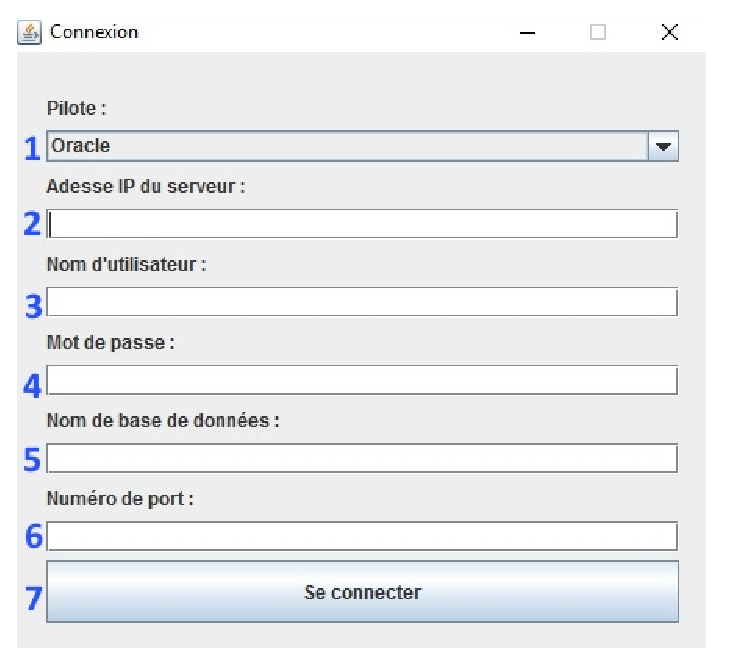
\includegraphics[width=10cm]{./images/manuel/se_connecter.eps}
\caption{\gls{ihm}* - Se connecter}
\label{se_connecter_gui}
\end{figure}

Pour se connecter, renseigner les différents champs présents dans la fen\^etre.

\begin{enumerate}
\item choix du \gls{sgbd}* (Oracle, MySQL).
\item Adresse IP du serveur où est stockée votre base de données.
\item Nom d'utilisateur utilisé pour vous connecter à votre base de données. 
\item Mot de passe utilisé pour vous connecter à votre base de données.
\item Nom de la base de données.
\item Numéros de port du serveur ou est stockée votre base de données.
\item Cliquer sur le bouton \textbf{se connecter} pour vous connecter au serveur.
\end{enumerate}

\subsection{Connexion aux serveurs de l'IUT}
Si vous êtes un étudiant de l'IUT de Montpellier.

\subsubsection{Oracle}
\begin{itemize}
\item SGBD : Oracle
\item Adresse IP : 162.38.222.149
\item Nom d'utilisateur : <nom-de-famille><première-lettre-du-prenom>
\item Mot de passe : <votre-INE>
\item Nom de la base de données : IUT
\item Numéros de port : 1521 \\
\end{itemize}

\subsubsection{MySQL}
\begin{itemize}
\item SGBD : MySQL
\item Adresse IP : 162.38.222.142
\item Nom d'utilisateur : <nom-de-famille><première-lettre-du-prenom>
\item Mot de passe : <votre-INE>
\item Nom de la base de données : <nom-de-famille><première-lettre-du-prenom>
\item Numéros de port : 3306
\end{itemize}

\section{Créer une table}
Dans le menu principal de l'application, cliquer sur le bouton \textbf{\gls{ldd} : créer tables} pour ouvrir la fen\^etre de création de tables (figure \ref{creer_table_gui}).

\begin{figure}[!h]
\centering
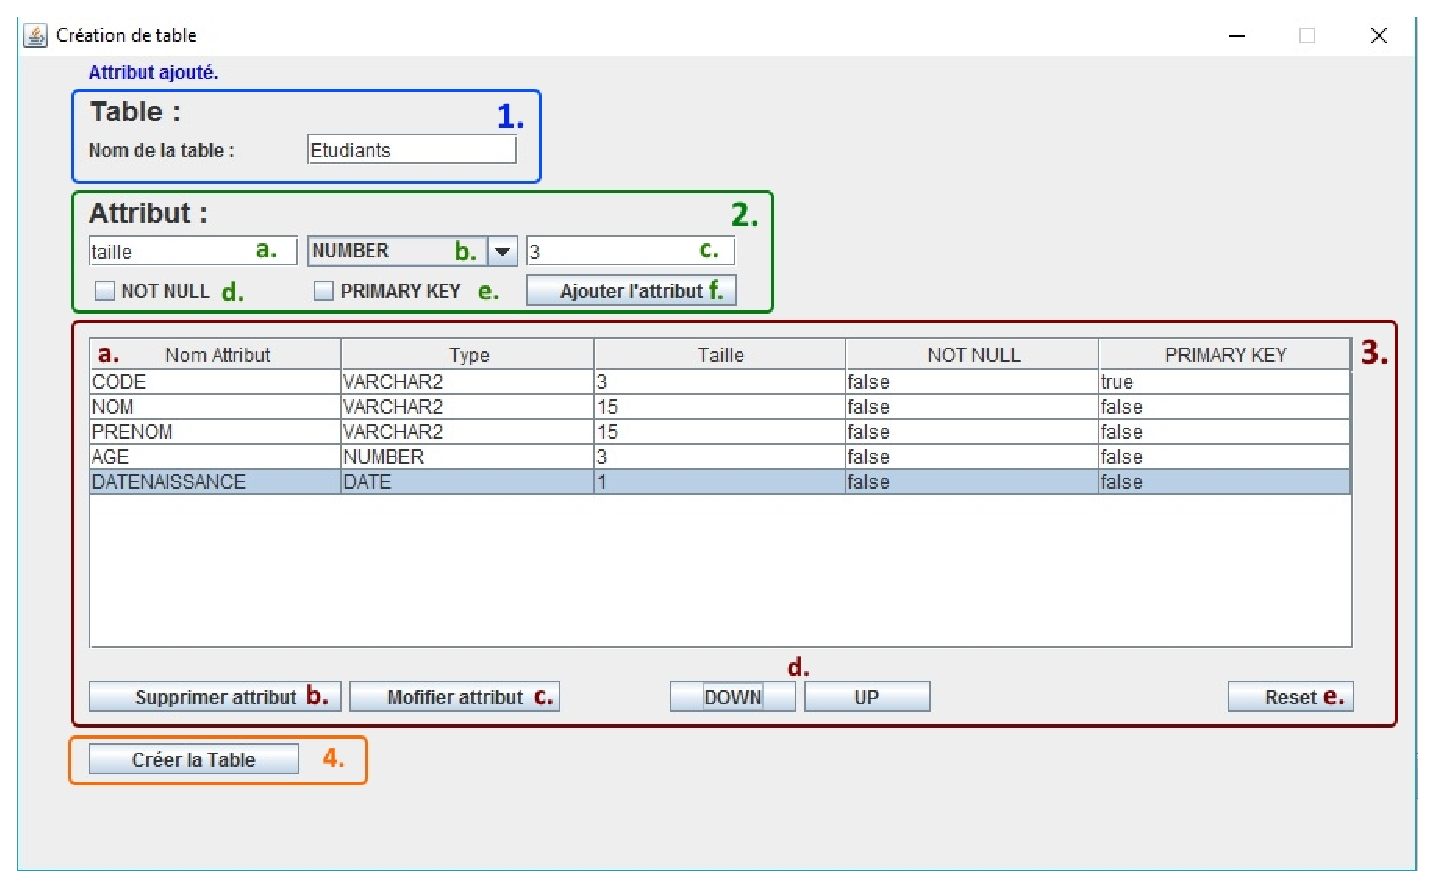
\includegraphics[width=14cm]{./images/manuel/creer_table.eps}
\caption{IHM - Créer table}
\label{creer_table_gui}
\end{figure}

\begin{enumerate}
\item Nom de ta table - \textit{ex : Etudiants}

\item Gestion des caractéristiques d'un attribut :
\begin{enumerate}
\item Nom - \textit{ex : codeEtudiant}
\item Type - \textit{ex : VARCHAR2}
\item Taille - \textit{ex : 15}
\item A cocher pour que l'attribut ne soit jamais null.
\item A cocher pour que l'attribut soit membre de la clée primaire de votre table.
\item Cliquer sur le bouton \textbf{Ajouter l'attribut} pour tenter d'ajouter un attribut à la table.
\end{enumerate}

\item Gestion des attributs ajoutés :
\begin{enumerate}
\item Tableau contenant les attributs ajoutés avec le bouton \textbf{Ajouter l'attribut}.
\item Cliquer sur le bouton \textbf{Supprimer l'attribut} pour supprimer l'attribut sélectionné dans le tableau.
\item Cliquer sur le bouton \textbf{Modifier l'attribut} pour modifier l'attribut sélectionné dans le tableau. 
Les caractéristiques de l'attribut sélectionné sont à modifier dans la zone de gestion des caractéristiques d'un attribut. 
Vous pouvez ensuite valider ou annuler votre modification.
\item Cliquer sur les boutons \textbf{UP/DOWN} pour modifier l'ordre des attributs dans le tableau. 
\item Cliquer sur le bouton \textbf{Reset} pour remettre à zéro la fen\^etre de création.
\end{enumerate}

\item Cliquer sur le bouton \textbf{Créer la table} pour créer la table.
\end{enumerate}


\section{Modifier une table}
Dans le menu principal de l'application, cliquer sur le bouton \textbf{LDD : modifier tables} pour ouvrir la fenêtre de modification de tables (figure \ref{modifier_table_gui}).


\begin{figure}[!h]
\centering
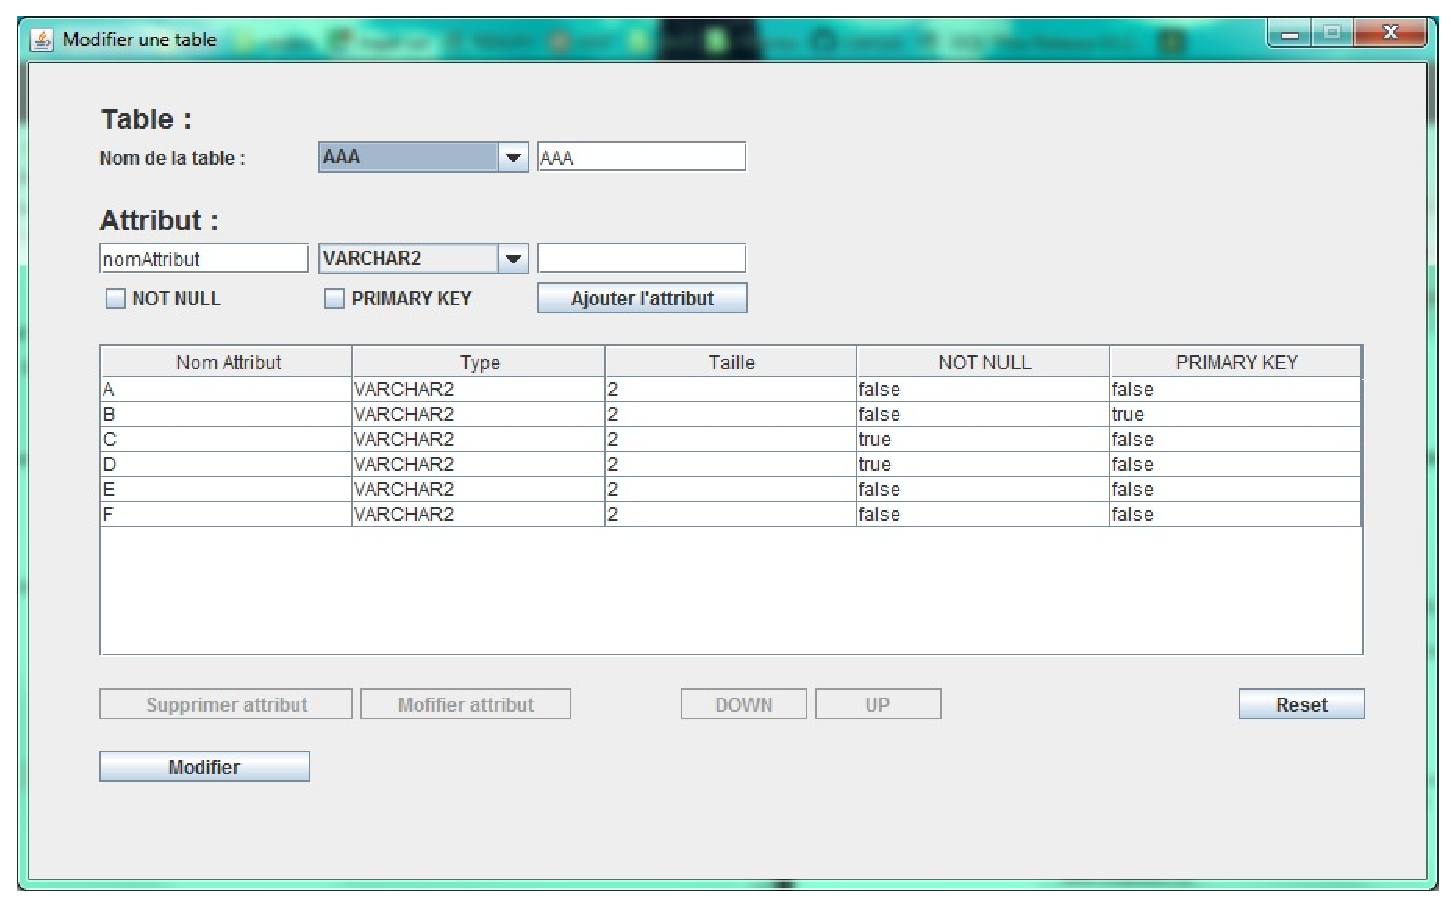
\includegraphics[width=10cm]{./images/manuel/modifier_tables.eps}
\caption{IHM - Modifier une table}
\label{modifier_table_gui}
\end{figure}

Cette fenêtre est identique à la fenêtre de création d'une table, à la différence qu'il est possible de sélectionner une table déjà existante dans la \bdd. 

Il est possible de modifier une table existante avec le bouton \textbf{modifier}, sans perdre de données mais il est possible que certaines soient perdues lors de la modification, notamment dans les cas suivants :
\begin{itemize}
\item suppression d'un attribut clée étrangère couplé avec un second attribut
\item modification du type de l'attribut pouvant altérer les données.
\end{itemize}





\section{Supprimer une table}
Dans le menu principal de l'application, cliquer sur le bouton \textbf{LDD : supprimer tables} ouvre la fen\^etre de suppression de tables (figure \ref{supprimer_table_gui}).

\begin{figure}[!h]
\centering
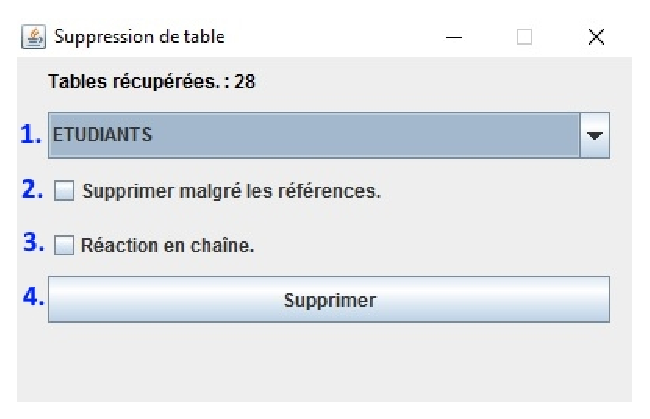
\includegraphics[width=8cm]{./images/manuel/supprimer_table.eps}
\caption{IHM - Supprimer une table}
\label{supprimer_table_gui}
\end{figure}

\begin{enumerate}
\item Choisir la table à supprimer.
\item A cocher pour supprimer sans prendre en compte les références des autres tables sur celle à supprimer.
\item A cocher pour supprimer la table sélectionnée puis toutes celles qui font référence à cette table et ceci récursivement.
\item Cliquer sur le bouton \textbf{Supprimer} pour tenter la suppression de la table.
\end{enumerate}

\section{Requ\^etes SQL}
Dans le menu principal de l'application, cliquer sur le bouton \textbf{\gls{sql}}* pour ouvrir la fen\^etre du mode requ\^etes SQL (figure \ref{sql_gui}).
\begin{figure}[!h]
\centering
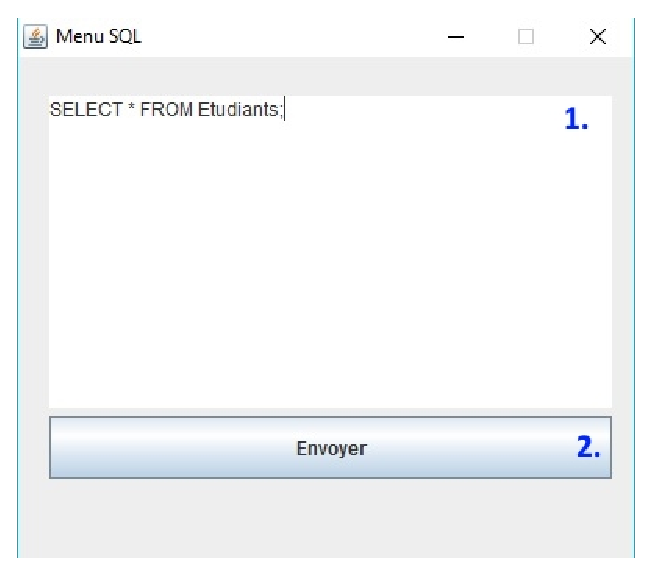
\includegraphics[width=6cm]{./images/manuel/sql.eps}
\caption{IHM - SQL}
\label{sql_gui}
\end{figure}

\begin{enumerate}
\item Ecrire la requ\^ete dans la zone de saisie - \textit{ex : SELECT * FROM Etudiants;} 
\item Cliquer sur le bouton \textbf{Envoyer} pour tenter d'exécuter la requ\^ete.
Une fenêtre (figure \ref{sql_result_gui}) s'ouvre indiquant le résultat de la requ\^ete si la syntaxe est correcte.
\end{enumerate}

\begin{figure}[!h]
\centering
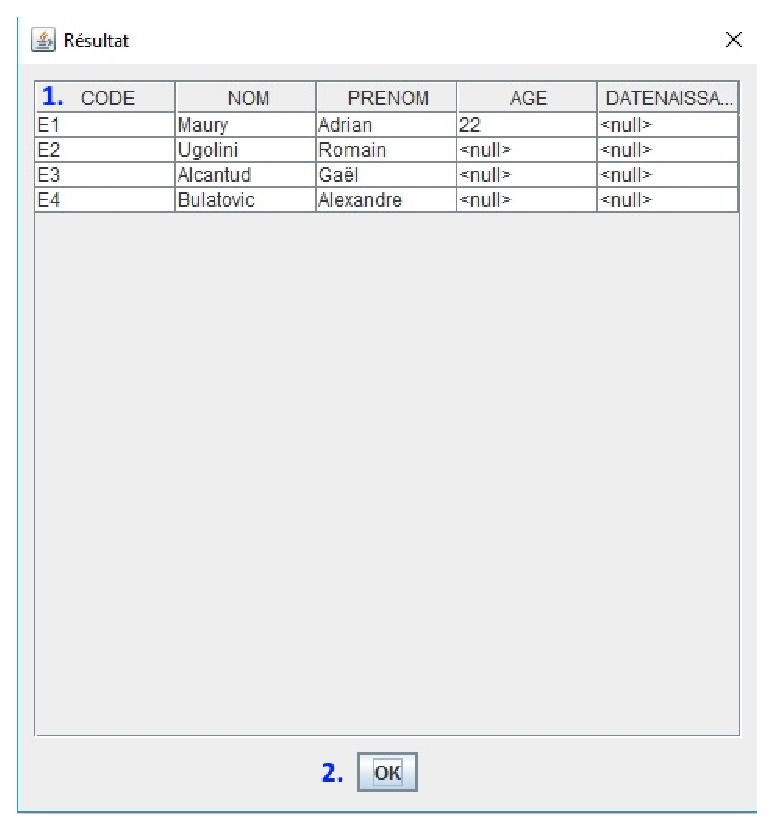
\includegraphics[width=8cm]{./images/manuel/sql_result.eps}
\caption{IHM - Résultat SQL}
\label{sql_result_gui}
\end{figure}

\begin{enumerate}
\item Résultat de la requ\^ete.
\item Cliquer sur le bouton \textbf{OK} pour fermer la fenêtre de résultat.
\end{enumerate}

\section{CRUD les tuples des tables}
Dans le menu principal de l'application, cliquer sur le bouton \textbf{\gls{crud}}* pour ouvrir la fen\^etre de gestion des \glspl{tuple}* des tables (figure \ref{crud_gui}).
\begin{figure}[!h]
\centering
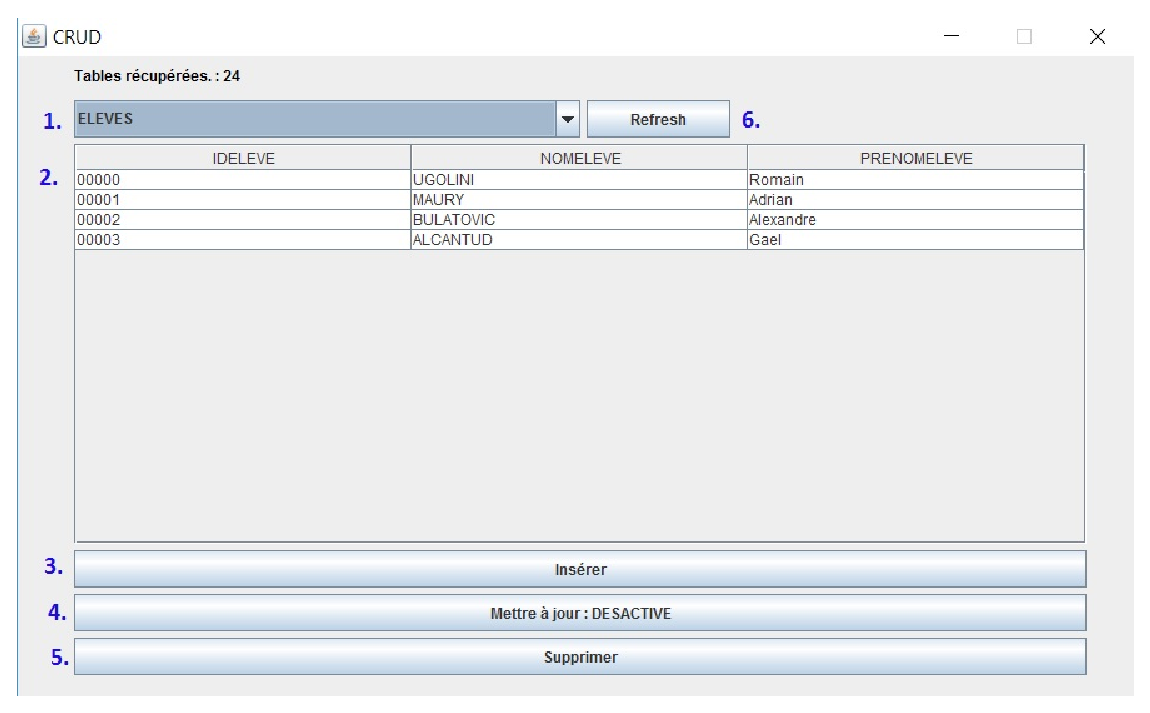
\includegraphics[width=12cm]{./images/manuel/crud.eps}
\caption{IHM - CRUD}
\label{crud_gui}
\end{figure}

\begin{enumerate}
\item Choisir la table.
\item Tableau contenant les différents tuples de la table sélectionnée.
\item Cliquer sur le bouton \textbf{Insérer} pour ajouter un tuple à la table. Il faut ensuite remplir les informations du nouveau tuple
dans la ligne vide qui s'est ajouté au tableau.
\item Cliquer sur le bouton \textbf{Mettre à jour} pour modifier un tuple de la table. Il faut ensuite modifer les informations du tableau et 
appuyer sur la touche entrée à chaque modification. Quitter le mode modification en cliquant une nouvelle fois sur le bouton \textbf{Mettre à jour}.
\item Cliquer sur le bouton \textbf{Supprimer} pour supprimer le tuple selectionné.
\item Cliquer sur le bouton \textbf{Refresh} pour rafraichir la vue dans le cas où des tuples ayant été supprimées sont affichées.
\end{enumerate}

\section{Ajouter et Supprimer des contraintes}

Dans le menu principal de l'application, cliquer sur le bouton \textbf{LDD : créer supprimer des contraintes} pour ouvrir la fen\^etre de création et suppression de contraintes unique et clées étrangères(figure \ref{contraintes_unique_gui}).

\begin{figure}[!h]
\centering
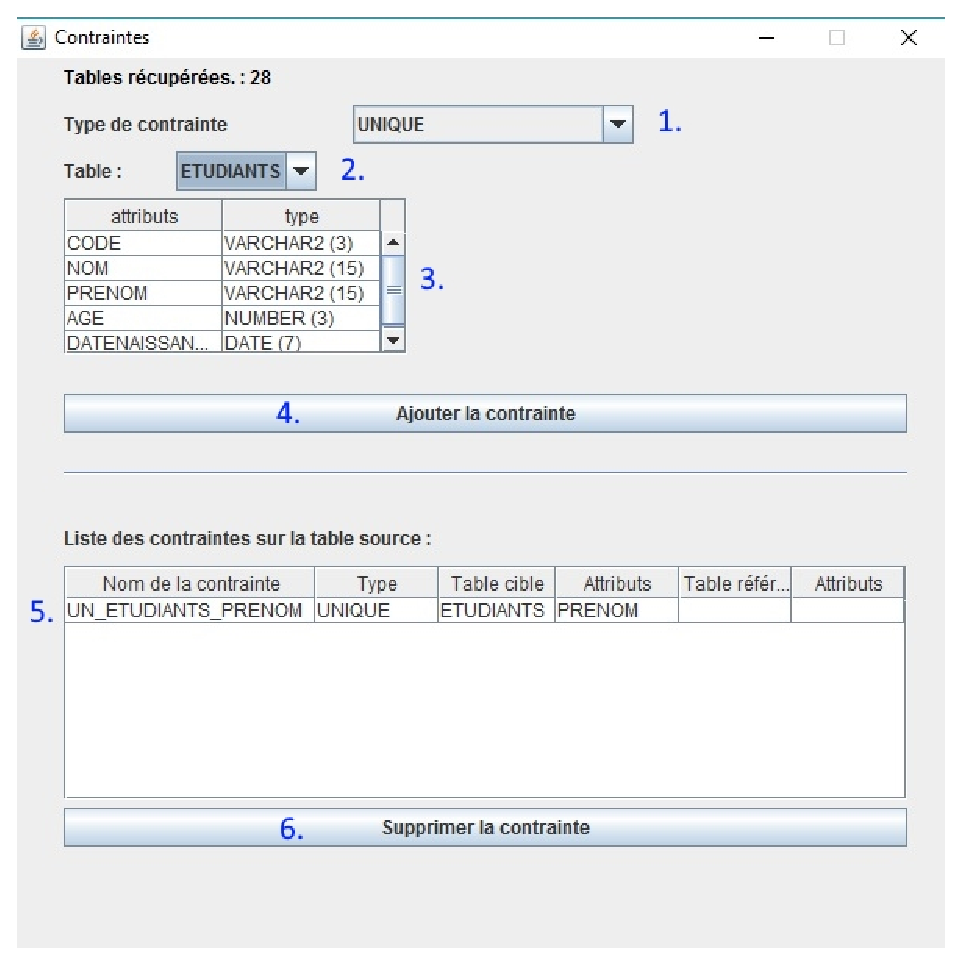
\includegraphics[width=12cm]{./images/manuel/contraintes_unique.eps}
\caption{IHM - Contraintes unique}
\label{contraintes_unique_gui}
\end{figure}

Pour créer une contrainte \textbf{unique} :
\begin{enumerate}
\item Choisir le type de contrainte à ajouter à votre table.
\item Choisir la table.
\item Tableau contenant les attributs de la table. Pour ajouter la contrainte il faut sélectionner des attributs dans ce tableau. La selection multiple de fait à l'aide de la touche CTRL.
\item Cliquer sur le bouton \textbf{Ajouter la contrainte} pour ajouter la contrainte à la table.
\item Tableau contenant les contraintes de la table source.
\item Cliquer sur le bouton \textbf{Supprimer la contrainte} pour supprimer la contrainte de la table et du tableau.
\end{enumerate}

Pour créer une contrainte \textbf{clée étrangère} ( FOREIGN KEY ) :\\
Même déroulement que pour une contrainte unique sauf pour les points 2 et 3 (figure\ref{contraintes_fk_gui}).

\begin{enumerate}
\item Choisir les tables source et destination pour la clée etrangère.
\item Tableaux contenant les attributs de la table source et de la table destination. Pour ajouter la contrainte il faut sélectionner des attributs dans ces tableaux. La selection multiple de fait à l'aide de la touche CTRL. Le nombre d'attributs sélectionnés dans la table source doit être le même que dans la table destination.
\end{enumerate}

\begin{figure}[!h]
\centering
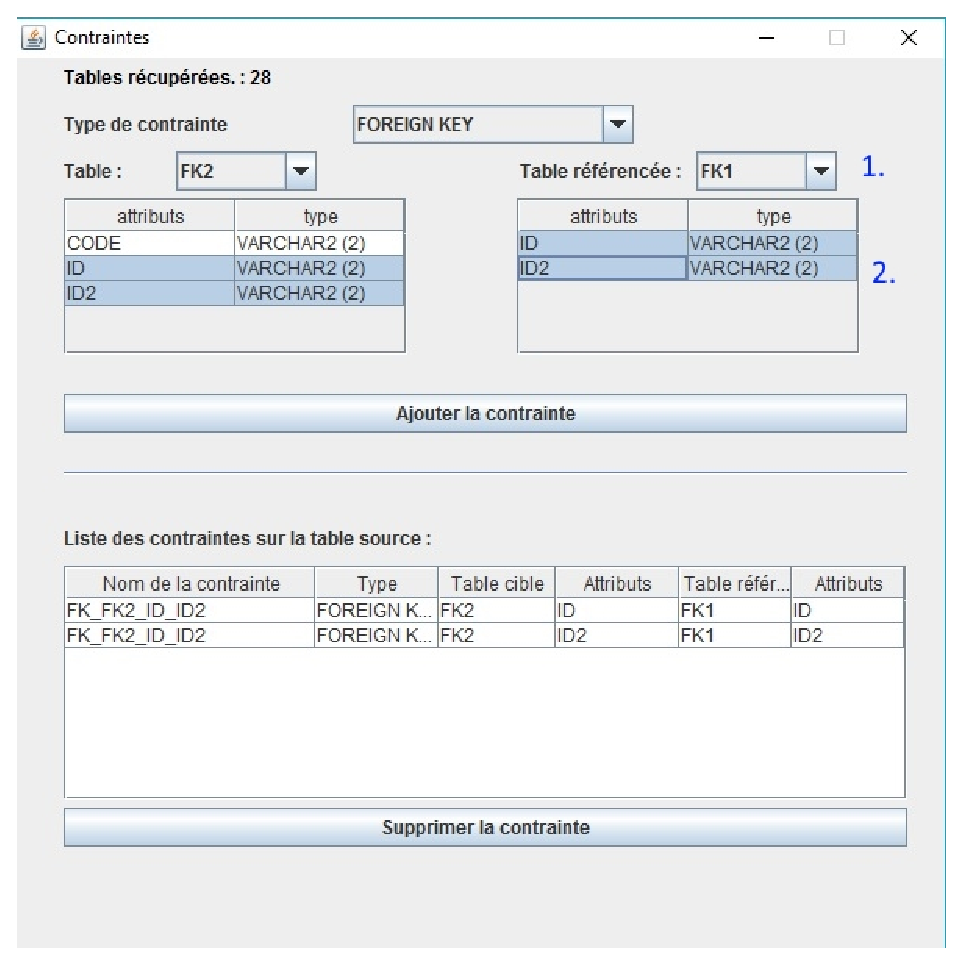
\includegraphics[width=12cm]{./images/manuel/contraintes_fk.eps}
\caption{IHM - Contraintes foreign key}
\label{contraintes_fk_gui}
\end{figure}


\section{Faire des requêtes graphiques : QBE*}

Dans le menu principal de l'application, cliquer sur le bouton \textbf{QBE : Requêtes} pour ouvrir la fenêtre de requêtes (figure \ref{qbe_gui}).

\begin{figure}[!h]
\centering
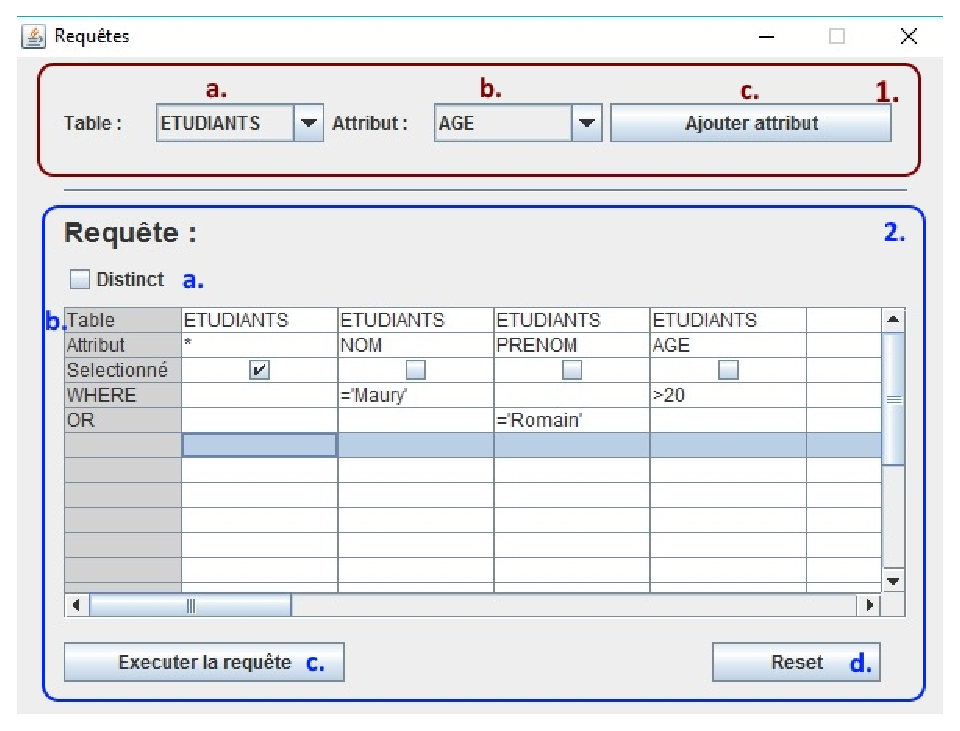
\includegraphics[width=12cm]{./images/manuel/qbe.eps}
\caption{IHM - Requêtes graphique (QBE)}
\label{qbe_gui}
\end{figure}

\begin{enumerate}
\item Ajouter un attribut à la requête :
\begin{enumerate}
\item Choisir la table.
\item Choisir l'attribut ou * pour selectionner tous les attributs.
\item Cliquer sur le bouton \textbf{Ajouter l'attribut} pour ajouter l'attribut à la requête.
\end{enumerate}
\item Modifier les caractéristiques de la requête :
\begin{enumerate}
\item A cocher pour qu'il n'y ai pas de doublon dans le résultat de la requête.
\item Tableau contenant les attributs utilisés dans la requête ainsi que les conditions de sélection pour la requête :
\begin{itemize}
\item Table : nom de la table cible.
\item Attribut : nom de l'attribut cible. ( * pour sélectionner tous les attributs de la table ).
\item Sélectionné : à cocher pour que l'attribut soit visible dans le résultat de la requête.
\item WHERE : condition de séléction sur un attribut. 
Plusieur conditions sur une même ligne correspondent à l'opérateur logique AND. \\
\textit{Ex (figure \ref{qbe_gui}) : nom = 'Maury' \textbf{AND} age>20}.\\
Plusieur conditions sur des lignes différentes correspondent à l'opérateur logique OR.\\
 \textit{Ex : (nom = 'Maury' AND age>20) \textbf{OR} prenom = 'Romain'}.\\
\end{itemize}
\item Cliquer sur le bouton \textbf{Executer la requête} pour executer la requête.
\item Cliquer sur le bouton \textbf{Reset} pour remettre à zéro la fenêtre.
\end{enumerate}
\end{enumerate}

La fenêtre de résultat de la requête s'ouvre. Cliquer sur le bouton \textbf{OK} pour fermer la fenêtre (figure \ref{qbe_result_gui}).

\begin{figure}[!h]
\centering
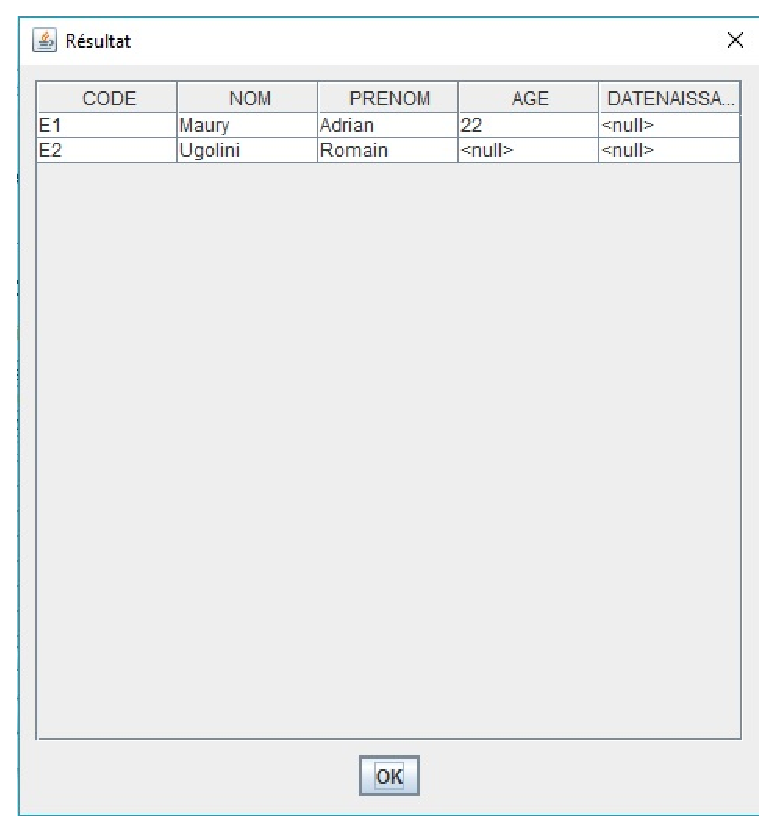
\includegraphics[width=12cm]{./images/manuel/qbe_result.eps}
\caption{IHM - Requêtes graphique (QBE) - Resultat}
\label{qbe_result_gui}
\end{figure}

\chapter{Rapport d'activité}
\section{Méthode de developpement}


\subsection{Cycle Itératif}
La méthode de développement pour le projet tuteuré est plus ou moins imposée. En effet pour pouvoir suivre l'avancement du projet, les tuteurs demandent aux étudiants d'utiliser un cycle itératif (figure \ref{cycle_iteratif}).

\begin{figure}[H]
\centering
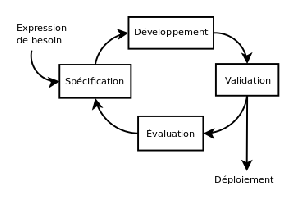
\includegraphics[width=8cm]{images/activite/cycle_iteratif.eps}
\caption{Schéma cycle Itératif}
\label{cycle_iteratif}
\end{figure}

\subsection{Outils de developpement}
Le choix du langage à utiliser était libre, nous avons donc opté pour un langage simple d'utilisation et ayant déjà fait ses preuves : \textbf{Java} (figure \ref{java_logo}).
\\
\\
\\

\begin{figure}[!h]
\centering
\includegraphics[width=8cm]{images/activite/javaLogo.eps}
\caption{Logo Java}
\label{java_logo}
\end{figure}


Nous avons choisi de travailler avec le logiciel \textbf{Éclipse} (figure \ref{eclipse_logo}), un \gls{IDE} pour développer en \textbf{Java}.

\begin{figure}[H]
\centering
\includegraphics[width=8cm]{images/activite/eclipseLogo.eps}
\caption{Logo Éclipse}
\label{eclipse_logo}
\end{figure}

\textbf{Éclipse} est disponible à l'IUT et libre.
La bibliothèque nous permettant de faire des \gls{ihm} est java.swing, un package Java documenté et expliqué par Oracle
\footnote{Tutoriel java.swing : \url{https://docs.oracle.com/javase/tutorial/uiswing/}}

\section{Planification}
Le projet a été découpé en sept itérations de durées variantes (d'une semaine à un mois) en fonction des périodes d'examens et de vacances. 
Chaque itération refactore le code et en ajoute.

\subsection{Itération 1 - 14/11/2016}

\subsubsection{Fonctionnalités et travail réalisé}
\begin{itemize}
\item Connexion à une base de données Oracle.
\item Mode requêtes SQL.
\end{itemize}

\subsubsection{Résultat}
L'utilisateur peut se connecter à une base de données mais il y a des problèmes au niveau des champs de saisies. 
Le mode requête SQL ne fonctionne pas parfaitement.
Cette itération n'a pas de grosse valeur ajoutée pour le client. 
Elle a surtout permis de poser les bases du travail en groupe en posant les bases des outils de collaboration.


\subsection{Itération 2 - 02/12/2016}
\subsubsection{Fonctionnalités et travail réalisé}
\begin{itemize}
\item Correction des bugs sur la fenêtre de connexion et sur le mode Requêtes SQL.
\item Création de tables.
\end{itemize}

\subsubsection{Résultat}
Les bugs signalés sont corrigés et la vue de création des tables fonctionne avec quelques bugs mineurs.
Cette itération est satisfaisante pour le groupe car les attentes ont été respectées.

\subsection{Itération 3 - 15/12/2016}
\subsubsection{Fonctionnalités et travail réalisé}
\begin{itemize}
\item Connexion à MySQL.
\item Correction des bugs sur la fenêtre de création des tables.
\item Suppression des tables.
\item Modification des tables.
\end{itemize}

\subsubsection{Résultat}
Les bugs signalés sont corrigés et la vue de suppression des tables fonctionne.
La modification des tables fonctionne partiellement.
Cette itération est mitigée car la valeur apportée au client n'était pas conséquente. 


\subsection{Itération 4 - 12/01/2017}
\subsubsection{Fonctionnalités et travail réalisé}
\begin{itemize}
\item Correction de bugs sur la fenêtre de modification des tables.
\item CRUD des tuples d'une table.
\end{itemize}

\subsubsection{Résultat}
La fenêtre CRUD fonctionne partiellement (fonctionnalité \textit{update} non-implantée) et quelques bugs sur l'insertion. 
La modification des tables fonctionne partiellement.
Cette itération est peu satisfaisante mais a permis une remise en question de notre organisation. 

\subsection{Itération 5 - 02/02/2017}
\subsubsection{Fonctionnalités et travail réalisé}
\begin{itemize}
\item Correction des bugs sur le CRUD et ajout de la fonctionnalité update.
\item Début de la refonte des classes métiers de l'application.
\end{itemize}

\subsubsection{Résultat}
La fenêtre CRUD fonctionne avec quelques bugs mineurs.
La refonte des classes métiers avait pour but de stocker les différentes informations des tables des bases de données et ainsi limiter les accès à celles-ci.
De plus, les classes métiers devaient permettre de gérer plus facilement le processus de modification des tables. 
La modification de table ne marche plus, mais la refonte des classes métiers va permettre de la faire fonctionner.
Cette itération est satisfaisante puisque la refonte des classes métiers simplifie beaucoup de choses. 

\subsection{Itération 6 - 09/02/2017}
\subsubsection{Fonctionnalités et travail réalisé}
\begin{itemize}
\item Correction des bugs sur la fenêtre CRUD.
\item Fin de la refonte des classes métiers de l'application.
\item Modification des vues de Creation-Supression-Modification des tables pour qu'elles collent aux classes métiers.
\item Création et supression des contraintes (uniques et clées étrangères).
\end{itemize}

\subsubsection{Résultat}
La fenêtre CRUD fonctionne avec quelques bugs mineurs.
La création et la suppression des tables fonctionnent avec les nouvelles classes métiers.
La création et la suppression des contraintes fonctionnent partiellement.
Cette itération est dans la continuité de l'itération 6. 

\subsection{Itération 7 - 20/02/2017}
\subsubsection{Fonctionnalités et travail réalisé}
\begin{itemize}
\item Correction des bugs sur la création et la suppression de contraintes ainsi que sur la fenêtre CRUD.
\item Faire des requêtes graphiques (QBE).
\item Modification de tables.
\item Refactoring.
\end{itemize}

\subsubsection{Résultat}

La modification des tables et le QBE fonctionnent.
La création et la suppression des contraintes fonctionnent avec quelques bugs mineurs.
Cette itération concerne surtout la correction des bugs et la rédaction du rapport. 


\section{Outils de collaboration}

\subsection{Gestionnaire de version}
Les premiers échanges que nous avons eus après l'attribution du sujet se sont concentrés sur le choix du gestionnaire de version que nous allions utiliser au cours du projet. Ce gestionnaire de version permet en autre de :
\begin{itemize}
\item Partager le code source de l'application.
\item Gérer des conflits lors de la modification simultanée d'un fichier.
\item Maintenir l'ensemble des versions d'un ou plusieurs fichiers.\\
\end{itemize}

Etant majoritairement habitué à utiliser Git, c'est vers un dép\^ot \textbf{Github} (figure \ref{github_logo}) que nous nous sommes tourné
\footnote{Site web GitHub : \url{https://github.com/}}.

\begin{figure}[H]
\centering
\includegraphics[width=8cm]{images/activite/githubLogo.eps}
\caption{Logo GitHub}
\label{github_logo}
\end{figure}



\subsection{Répartition des tâches}
Au cours de leurs formations antérieures, certains membres du projet ont utilisé l'outil de gestion de projet \textbf{Trello} (figure \ref{trello_logo}). 
C'est pourquoi nous avons utilisé cet outil pour répartir les tâches.\\

\begin{figure}[H]
\centering

\includegraphics[width=8cm]{images/activite/trelloLogo.eps}
\caption{Logo Trello}
\label{trello_logo}
\end{figure}

\textbf{Trello} permet de découper en \textit{tickets} les différentes t\^aches à réaliser. Ces tickets peuvent \^etres déplacés par les membres du projet dans différentes catégories :

\begin{itemize}
\item \textbf{TODO} - les t\^aches qu'il restent à faire. 
\item \textbf{DOING} - les \^aches en cours de développement.
\item \textbf{TESTS} - les t\^aches en cours de test.
\item \textbf{DONE} - les t\^aches qui sont terminées.\\
\end{itemize}

Chaque membre choisit un ticket dans la partie TODO et le déplace dans DOING. 
Puis lorsqu'il a terminé de développer la fonctionnalité, le ticket va dans TEST et pour finir dans DONE.

\subsection{Communication}
Les outils de communication ont évolué au cours du projet. Nous avons tout d'abord utilisé naturellement la messagerie instantanée que propose \textbf{Facebook}. 
Cette messagerie simple, permet de partager des images ainsi que des documents.
Cependant nous souhaitions pouvoir discuter à l'oral ce que ne permet pas facilement la messagerie de Facebook. 
C'est pour cette raison que nous avons migré sur le logiciel \textbf{Discord} (figure \ref{discord_logo}) qui permet, en plus de la messagerie et de l'échange de documents, de discuter à l'oral ce qui a grandement facilité notre communication.

\begin{figure}[!p]
\centering

\includegraphics[width=10cm]{./images/activite/discordLogo.eps}
\caption{Logo Discord}
\label{discord_logo}
\end{figure}

De plus, nous avons installé un BOT sur le Discord, lié a GitHub, qui écrit un message lors d'une modification du dép\^ot git (figure \ref{bot_discord}).

\begin{figure}[!p]
\centering

\includegraphics[width=10cm]{./images/activite/bot_discord.eps}
\caption{Message du BOT Discord lié à GitHub}
\label{bot_discord}
\end{figure}



\subsection{Partage de documents}
Tout au long du projet, nous avons produit différents documents qu'il nous a fallu stocker dans un endroit facile d'accès pour tous. 
Nous avons donc créé un dossier sur un \textbf{Google Drive} (figure \ref{googledrive_logo}) et l'avons partagé aux membres du groupe. Ce Drive nous a permis d'échanger et stocker des diagrammes, des pdfs, des documents texte, des maquettes pour les \glspl{ihm}* ainsi que d'autres fichiers que nous voulions conserver.

\begin{figure}[!p]
\centering

\includegraphics[width=10cm]{./images/activite/googleDriveLogo.eps}
\caption{Logo Google Drive}
\label{googledrive_logo}
\end{figure}





\backmatter

\chapter{Résumé}
\textbf{IDB} est un logiciel gratuit permettant d'utiliser un SGBD* au moyen d'une interface graphique. Son interface est intuitive et permet à un utilisateur, même non informaticien, de manipuler très facilement des tables et les données qu'elles contiennent, mais aussi d'effectuer des requêtes simples (en allant jusqu'aux jointures) sans se soucier du langage SQL*.
\\
Le logiciel est entièrement codé en langage Java (nécessite au minimum JRE* 1.7) et se base sur la bibliothèque JDBC* pour réaliser la communication avec la base de données. Il est entièrement compatible avec les système de gestion de base de données Oracle Database et MySQL.
\bigbreak
Mots clés : base de données, JAVA, JDBC, SQL, interface graphique, Oracle, MySQL, QBE

\bigbreak
\rule{\linewidth}{0.4pt}
\bigbreak

\textbf{IDB} is a free software intended to handle the administration of a database management system with the use of a GUI*. Its use is intuitive and allow non-IT people to manage tables and their data, but also to perform simple queries (even join clause) without having to know SQL*.
\\
This software is written in Java language (requires JRE* 1.7+) and uses the JDBC* tool from Java language to achieve communication with the database management system. It's fully compatible with Oracle Database and MySQL.
\bigbreak
Keywords : database, JAVA, JDBC, SQL, graphical user interface, Oracle, MySQL, QBE


\end{document}
